\documentclass[a4paper,10pt]{article}
\usepackage[utf8]{inputenc}

\usepackage{amstext, amsfonts, amsmath, amsbsy, amssymb}
\usepackage[paper=a4paper,marginparwidth=0mm,marginparsep=0mm,margin=20.5mm,includemp]{geometry}
\usepackage{tikz}
\usepackage{blkarray}

%Math symbols
\DeclareMathOperator{\Poisson}{Poisson}
\DeclareMathOperator{\Multinom}{Multinom}
\DeclareMathOperator{\logit}{logit}
\DeclareMathOperator{\cov}{cov}
\def\P{\mathbb{P}}
\def\E{\mathbb{E}}
\def\M{\boldsymbol{M}}
\def\I{{\cal I}}
\def\x{\boldsymbol{x}}
\def\d{\boldsymbol{d}}
\def\bnu{\mbox{\boldmath $\nu$}}
\def\bP{{\bf P}}
\def\R{{\bf R}}
\def\dd{\mathrm{d}}


\linespread{1.25}



%opening
\title{Inferring the presence of metabolites}

\begin{document}

\maketitle

\section{Idea and concept}
	
	We seek to infer the presence or absence of $M$ metabolites in $S$ species. We denote by $x_{sm}$ whether metabolite $m=1,\ldots,M$ is present ($x_{sm}=1$) or absent ($x_{sm}=0$) in species $s=1,\ldots,S$. To infer the full vector $\x=(x_{11}, \ldots, x_{1M},\ldots,x_{SM})$, we assume that related species share a similar set of metabolites and that metabolites related in their synthesis share a similar distribution across species. 
	Let $\P(x_{sm}=1|y_{sm})=y_{sm}$ be the probability with which metabolite $m$ is present in species $s$. We then assume that
	
	\begin{equation*}
	 \logit y_{sm} = \mu_m + \epsilon_{sm}
	\end{equation*}
	
	where $\mu$ is a metabolite-specific intercept and $\epsilon_{sm}$ is normally distributed with mean 0 and co-variance $\cov(\epsilon_{sm},\epsilon_{s'm'})=\alpha \sigma_{ss'} + \beta \sigma_{mm'}$ between each combination of species and metabolite. Here, $\sigma_{ss'}$ and $\sigma_{mm'}$ are known measures of covariance between species $s$ and $s'$ and between metabolites $m$ and $m'$, respectively, and $\alpha$ and $\beta$ are positive scalars.
	
	We consider two sets of data informative about $\x$: i) Presence-absence data obtained with mass-spectrometry and ii) presence-only reports of specific metabolites in specific specie. Let $\d_{sj}=(d_{sj1}, \ldots, d_{sjM})$ be the presence-absence vector of each metabolite $m$ obtained with mass-spectrometry run $j=1,\ldots,J_s$ performed on species $s$. Assuming a false-positive and false-negative error rates $\epsilon_{01}$ and $\epsilon_{10}$, respectively, we have
	
	\begin{equation*}
	 \P(\d_{sj}|\x, \epsilon_{01}, \epsilon_{10}) = \prod_m \left[ x_{sm}\left(\epsilon_{10}^{1-d_{sjm}}(1-\epsilon_{10})^{d_{sjm}}\right) + (1-x_{sm})\left( \epsilon_{01}^{d_{sjm}}(1-\epsilon_{01})^{1-d_{sjm}}\right)\right].
	\end{equation*}
	
	To model the presence only data, it must be put in relation to the expected research effort. Let $p_{sm}$ denote the known number of presence-only reports for metabolite $m$ in species $s$ and $n_{sm}$ the unknown number of research projects that aimed at discovering metabolite $m$ in species $s$. Assuming a false-positive and false-negative error rates $\pi_{01}$ and $\pi_{10}$, respectively, we have
	
	\begin{equation*}
	 \P(p_{sm}|n_{sm}, \pi_{01}, \pi_{10}) = 
	\end{equation*}
	
	
	We would have the covariance matrix such as :
	
	\begin{equation}
		\cov (\epsilon_{smt}, \epsilon_{s'm't'}) = \alpha \sigma_{ss'}^P + \beta \sigma_{mm'}^M + \gamma \sigma_{ss'}^E + \ldots
	\end{equation}
	
	With $P$ the phenotype between two species, $E$ an environment factor between two species and $M$ the TODO 

\section{DAG scratch}
	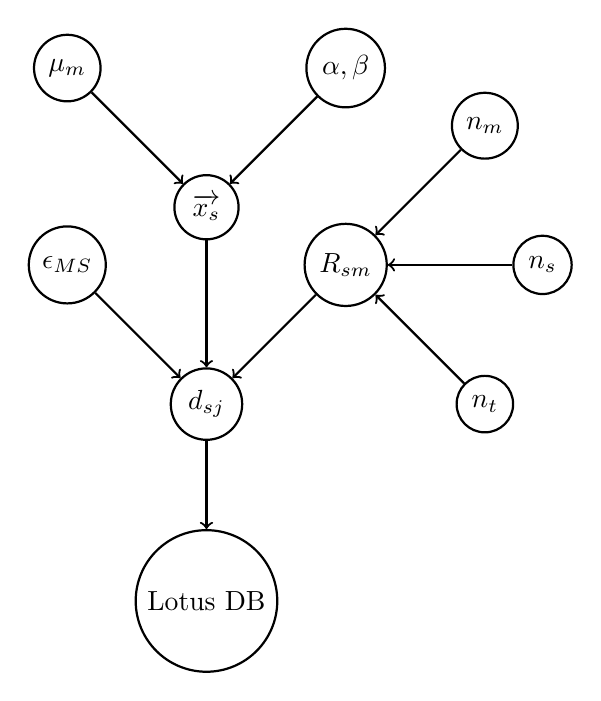
\begin{tikzpicture}[node distance={25mm}, thick, main/.style = {draw, circle}]
		\node[main] (1) {$d_{sj}$}; 
		\node[main] (2) [above left of=1] {$\epsilon_{MS}$};
		\node[main] (3) [above right of=1] {$R_{sm}$}; 
		\node[main] (4) [above of=1] {$\overrightarrow{\boldmath{x_s}}$};
		\node[main] (5) [above left of=4] {$\mu_m$}; 
		\node[main] (6) [above right of=4] {$\alpha, \beta$};
		\node[main] (7) [below of=1] {Lotus DB};
		\node[main] (8) [above right of=3] {$n_m$};
		\node[main] (9) [ right of=3] {$n_s$};
		\node[main] (10) [below right of=3] {$n_t$};
		
		\draw[->] (5) -- (4);
		\draw[->] (6) -- (4);
		\draw[->] (4) -- (1);
		\draw[->] (2) -- (1);
		\draw[->] (3) -- (1);
		\draw[->] (1) -- (7);
		\draw[->] (8) -- (3);
		\draw[->] (9) -- (3);
		\draw[->] (10) -- (3);
	\end{tikzpicture} 

\section{Ideas scratch}
	\begin{blockarray}{cccc}
		& $L_{sm} = NA$ & $L_{sm} = 1$ \\
		\begin{block}{c(ccc)}
			$x_{sm}=0$ & $1$ & $0$  \\
			$x_{sm}=1$ & $1-R_{sm}$ & $R_{sm}$ \\
		\end{block}
	\end{blockarray}


	With $x_{sm}$ a molecule present or not present in a specific species. $L_{sm}$ the presence or absence of a molecule in a species that is present or not in the Lotus database. Finally, $R_{sm}$ the research effort made for that specific molecule. $R_{sm}$ being a function of the number of papers made on a specific molecule or species : $f(n_s, n_m)$. 
\end{document}
